\documentclass[titlepage]{article}
\usepackage{fancyhdr}
\usepackage{graphicx}
\usepackage[hidelinks]{hyperref}
\pagestyle{fancy}
\title{Computer Workshop\\Final Project}
\author{AmirAbas Eshghi / 402521414}
\date{Due: 06 Bahman, 1402}
\begin{document}
	\maketitle
	\tableofcontents
	
	\newpage
	\section{Git and Github}
	\subsection{Repository Initialization and Commits} 
	\begin{enumerate}
	  \item I make a public repository with name Final project and then clone it to my local PC.
	  \item After that i  make a new folder with name Final Project and then i (cd) in it. 
	  \item when I cd in it , I create a new folder with (mkdir) with name .github and near taht I create a main.tex file with (touch) command.
  \end{enumerate}
  \subsection{GitHub Actions for LaTeX Compilation}
  \begin{enumerate}
  	\item I copied the text in main.yml file and then I see some bugs in that. 
  	\item The first bug is that to when I send it to my GitHub by tag to compile it in GitHub , it gives me a wrong action that is for my Latex code.
  	\item After debugging my code and fixing its bugs , it compiled truly 
  \end{enumerate}
  




  \newpage
	\section{Exploration Tasks}
	\subsection{Vim Advanced Features}
	\begin{enumerate}
	  \item Tabbed editing: Vim allows you to have several files open in different tabs, which can be initiated using the ":tabe <filename>"  command. This enables tab expansion mode to make it easy to find files and allows you to switch between tabs using "gt" and "gT".
	  \item Text manipulation: Vim provides various commands for manipulating text, such as changing the case of text using the "gU" command with movement commands. 
	  \item Block operations: Vim allows you to perform operations on a block of text, such as commenting or uncommenting a block of code. To comment a block of code, position the cursor over the block and use the ":normal! I" command to add a comment character at the beginning of each line. The reverse operation to uncomment the block works similarly.
	 \end{enumerate}
	
	\subsection{Memory profiling}
	\subsubsection{Memory Leak}
	Memory leaks occur when a program allocates memory but fails to free it when it's no longer needed , resulting in a waste of system resources. Memory leaks can happen due to various reasons :
	\begin{enumerate}
		\item Forgetting to free memory : This is the most common cause of memory leaks. When a program allocates memory using a function like malloc() or realloc() and calloc() , it's the responsibility of the programmer to free that memory when it's no longer required using a function like free() or delete().
		\item Using global variables: When a program uses global variables to store data, it can lead to memory leaks if the data is not properly initialized or freed. This is because global variables are allocated at program startup and remain in memory until the program terminates.
		\item Using recursive functions: Recursive functions can cause memory leaks if they're not implemented correctly. This is because each recursive call allocates memory for its own stack frame, which can lead to a significant amount of memory being allocated if the function is called repeatedly.
	\end{enumerate}
	
	\subsubsection{Memory profilers}
	Valgrind is a tool for memory debugging, leak detection, and profiling in C and C++ programs. It detects memory allocation issues and provides detailed reports on the lines of code causing the leaks, with call stack information. This helps developers identify and fix memory-related problems in their code.
	
	\subsection{GNU/Linux Bash Scripting}
	\subsubsection{fzf}
	\begin{enumerate}
		\item Fuzzy searching is a search technique that enables users to locate items that have a partial match with their search query instead of requiring an exact match. It assists users in finding what they're looking for even if they're uncertain about the precise spelling, syntax, or other specifics of the search query. Fuzzy searching uses algorithms to compare the search query with the items being searched, taking into account factors such spelling errors, typos, and similarities in meaning, to return a list of items that are close matches to the search query. \\
		\item The command "ls | fzf" performs a fuzzy search on the list of files in the current directory. This command is a quick and easy way to search through the files in your current directory using fuzzy matching.
	\end{enumerate}
	
	\subsubsection{Using fzf to find your favorite PDF}
	\begin{enumerate}
		\item To list the directory of all the files with the extension .PDF, you can use the "fd" command with the "-t f" (for files) and "-e pdf" (for files with the .pdf extension) options:
			\begin{verbatim}
			fd -t f -e pdf
			\end{verbatim}
		\item To use "fzf" to select a PDF from the list of files gathered above, you can use the "fzf" command with the "--preview" option to preview the contents of the file and the "--bind" option to bind the enter key to open the selected file with a PDF viewer:
			\begin{verbatim}
			fd -t f -e pdf
			\end{verbatim}
	\end{enumerate}

	\subsubsection{Opening the file using Zathura}
	To open the selected PDF file using Zathura , you can use the following command:
	\begin{verbatim}
	zathura "$(fd -e pdf | fzf)"
	\end{verbatim}
  
  
  \newpage
	\section{Git and FOSS}
	\subsection{README.md}
	You can see detailed information about the project in the \href{https://github.com/AmirAbasEshghi/Final_project/blob/main/README.md}{README.md} file.

	\subsection{Issues}
	\begin{figure}[ht]
	\centering
	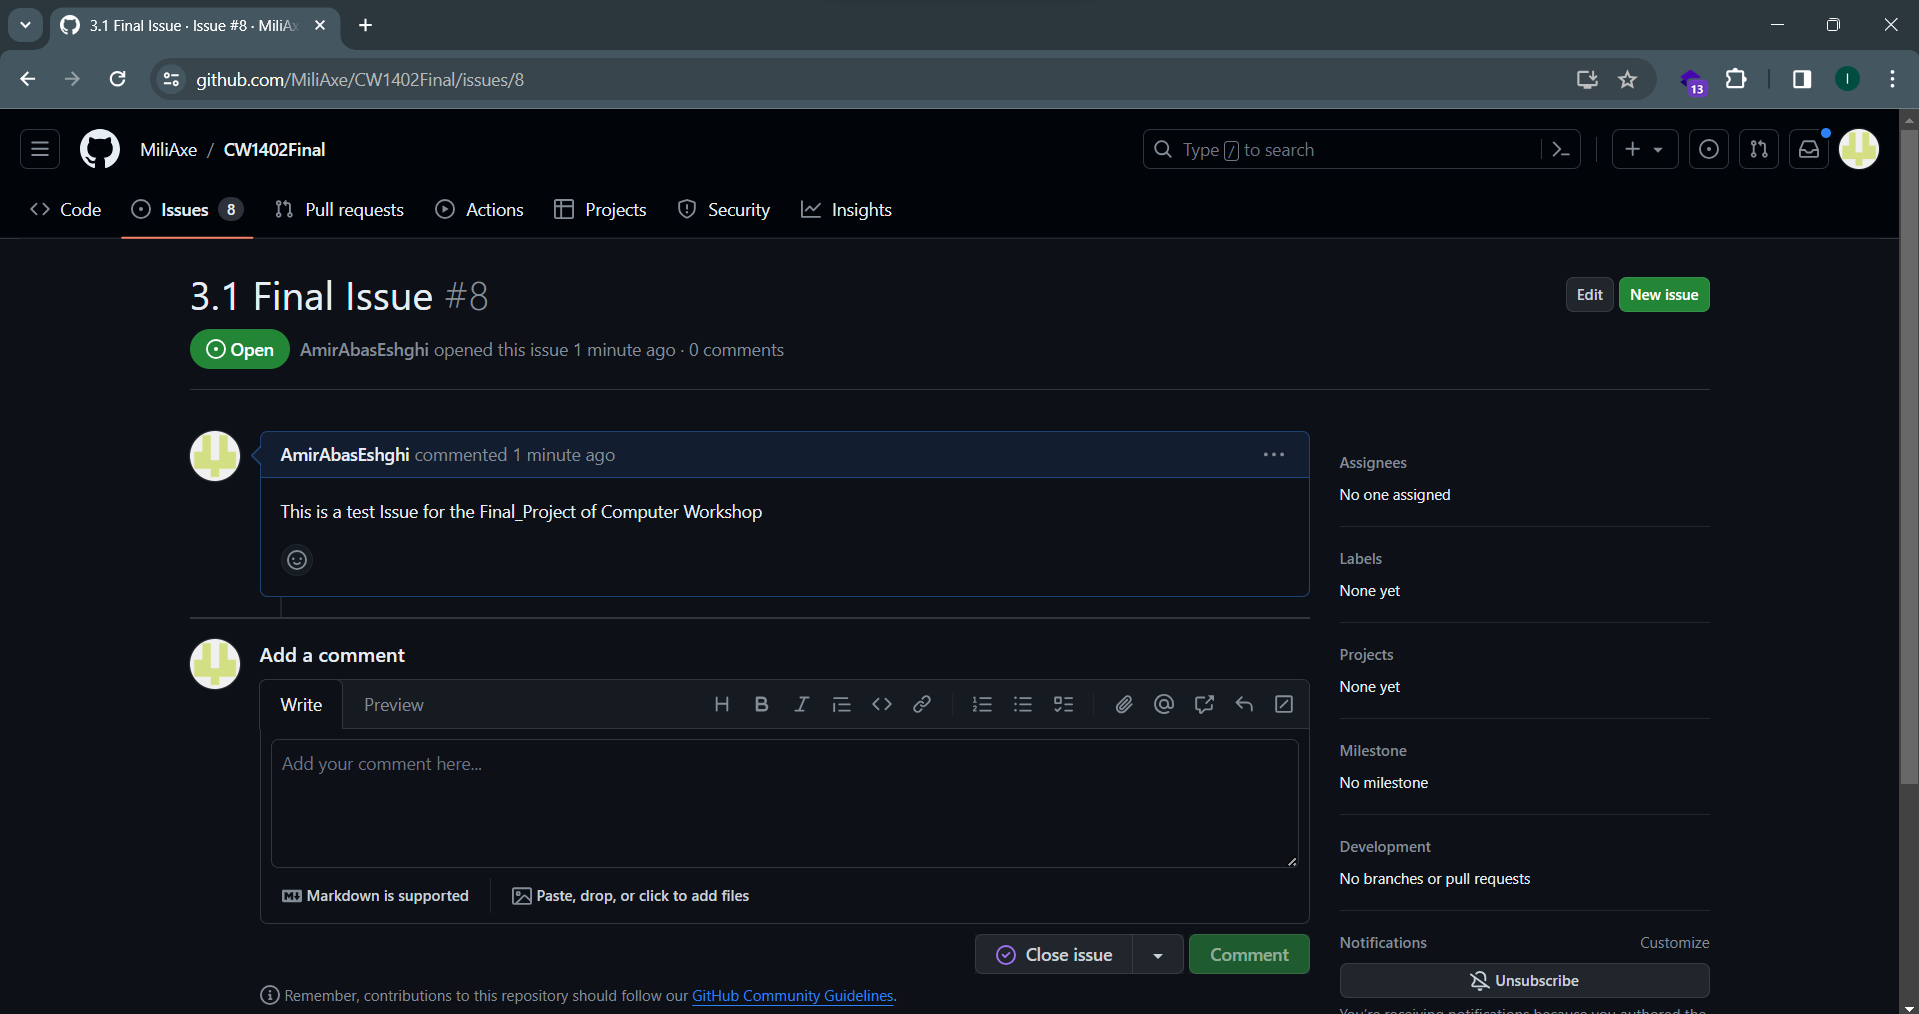
\includegraphics[width=1\textwidth]{issue.png}
	\caption{Issue screenshot CW}
	\end{figure}

\end{document}
